\chapter{Introducción} 


\begin{flushright}
\textit{''No mires al sol con inocencia, pues en su núcleo de fuego no late la vida, sino una conciencia antigua y soñolienta que, al despertar, nos reducirá a polvo.''}

-H. P. Lovecraft
\end{flushright}

Desde la antiguedad, el ser humano ha buscado respuestas a preguntas relacionadas con nuestra posición en el universo y sobre el funcionamiento de su entorno. El Sol, como fuente de luz y calor, se ha considerado como una deidad en el pasado y ha alimentado la curiosidad del hombre, como en \cite[e.g.,]{2010anaxagoras} en donde se dice que Anaxágoras de Clazómenas (c. 500 – 428 a.C.) creó una teoría en la que afirma que el Sol es una masa de metal incandescente y que no era el carro del dios Helios, como se creía entonces. Ya en la actualidad, gracias a avances en la ciencia y en la tecnología, se ha desarrollado un enorme marco teórico con el fin de entender el funcionamiento del Sol, encontrandose en el camino con diferentes eventos solares como lo son las \ac{SF}\index{Solar Wind}, los eventos de \ac{CME}\index{Coronal Mass Ejection}, las \ac{Sunspots}\index{Sunspots} que fueron utilizadas por Galileo en 1612, \cite[e.g.,]{vaquero-2009}, para determinar el periodo de rotación del Sol sobre su propio eje (27 días) mencionado en su publicación \textit{Istoria e dimostrazione intorno alle macchie solari} (Historia y demostraciones sobre las manchas solares). 

También, se ha encontrado que el Sistema Solar está inmerso en un medio gaseoso interplanetario, \cite{1951ZA.....29..274B, parker-1958}, que luego fue determinado como \ac{SW}\index{Solar Wind}, el cual es el culpable del clima espacial en conjunto con los eventos de \ac{CME}\index{Coronal Mass Ejection} y de \ac{SF}\index{Solar Flare}, así como de ayudar a determinar las fronteras del Sistema Solar, \cite{stone-2013}, es decir, los límites de la Heliosfera.

\section{Capas del Sol}

%Explicar lo que es la zona convectiva y fostosfera, el campo poloida y el campo toroidal, hablar de las diferentes zonas del Sol.


\section{Rotación diferencial del Sol}
Hoy sabemos que el Sol está hecho de \index{plasma}, un estado de la materia en donde los átomos se encuentran ionizados debido a las altas energías a las que se encuentra el material (....K), dando como resultado un gas de partículas ionizadas a altas temperaturas. El plasma es el cuarto estado de la materia, después del estado gaseoso, líquido y sólido, compuesto por un fluido de partículas cargadas o iones con propiedades electromagnéticas, estos iones llegaron a ese estado debido a las altas temperaturas en las que se encuentran. Es decir, que la materia va cambiando de fase a medida que se aumenta de temperatura partiendo del estado sólido, pasando por el líquido y el gaseoso hasta llegar al plasma. El Sol está conformado por plasma \cite[e.g,][]{cermak-2025} el cual presenta una composición de núcleos de oxígeno, nitrógeno, carbono, helio, deuterio, hidrógeno entre otros \cite[e.g.,][]{asplund-2009}. El Sol, al ser una acumulación de plasma, presenta una \index{rotación diferencial}, la cual indica que no todas las partes en su superficie tienen la misma velocidad angular, por lo que se generan regiones con diferentes velocidades tangenciales a la superficie de forma que el Sol no rota como un cuerpo sólido, sino que la velocidad tangencial es más grande en el ecuador que en los polos. Esto ocurre porque las capas externas (convectiva y fotosfera) están compuestas de gas ionizado (fluido), por lo que cada región en su superficie es independiente de las demás.

Esta rotación diferencial es la que alimenta el ciclo solar generando estructuras como \ac{Sunspots}\intex{Sunspots}, \acp{CME}\index{Coronal Mass Ejection}, \acp{SF}\index{Solar Flare} entre otros, es decir que alimenta el \index{Dinamo solar}. Es el proceso que explica la generación y mantenimiento del campo magnético del Sol. Este campo magnético, que varía a lo largo del ciclo solar, es resultado del complejo movimiento del plasma solar conductor y la rotación diferencial del Sol. El dinamo solar funciona gracias a la convección (transferencia de calor) y a la rotación diferencial del Sol, ya que al estar formado por plasma en movimiento genera corrientes eléctricas internas que a su vez generan campos magnéticos, por lo que la forma de las lineas de campo magnético abiertas y cerradas dependen de las corrientes internas del plasma. El movimiento del plasma en presencia de un campo magnético preexistente, induce nuevas corrientes, amplificando el campo magnético inicial, este proceso se conoce como efecto dinamo.

La rotación diferencial convierte el campo poloidal (como un dipolo) en campo toroidal (horizontal, como bandas alrededor del Sol).

La corona solar, al estar compuesta de hidrógeno ionizado (plasma) a altas temperaturas, mayores a los $10^{6}$K, bajas densidades al rededor de $10^{-16}g~cm^{-3}$ se expande a velocidades supersónicas formando la espiral de Parker, \cite[e.g.,]{lugaz-2005}.

%hablar más de la convección

\subsection{Manchas Solares}
Una mancha solar es una región oscura de alta actividad magnética en la superficie del Sol, es relativamente más fría que las demás regiones, puesto que el intenso campo magnético presente hace que el calor interno del Sol no alcance la superficie. Las manchas solares son un indicador de la actividad solar, y su número y tamaño varían a lo largo del ciclo solar como lo muestra \cite[e.g.,][]{hathaway-2015}, además de estar relacionadas con la producción de \ac{CME}\index{Coronal Mass Ejection}

\subsection{Llamaradas solares}
Las Solar Flares o llamaradas solares son procesos ocurridos en la corona solar debido a los bucles solares, además de ser impulsadas por la reconexión magnética que ocurre cuando una línea de campo magnético de un bucle solar presenta una torcedura que hace que se rompa y se reconecte de forma agresiva liberando una enorme cantidad de energía magnética en forma electromagnética (desde el rango de las ondas de radio hasta el de los rayos gamma) después de haber calentado mucho más el material presente en esa región, como lo menciona \cite[e.g.,][]{SolarFlares} y a su vez acelerando partículas de forma impulsiva, lo que significa que las acelera en un instante de tiempo relativamente corto.

\subsection{Eyecciones de masa coronal (CMEs)}


\begin{figure}[H]
    \centering
    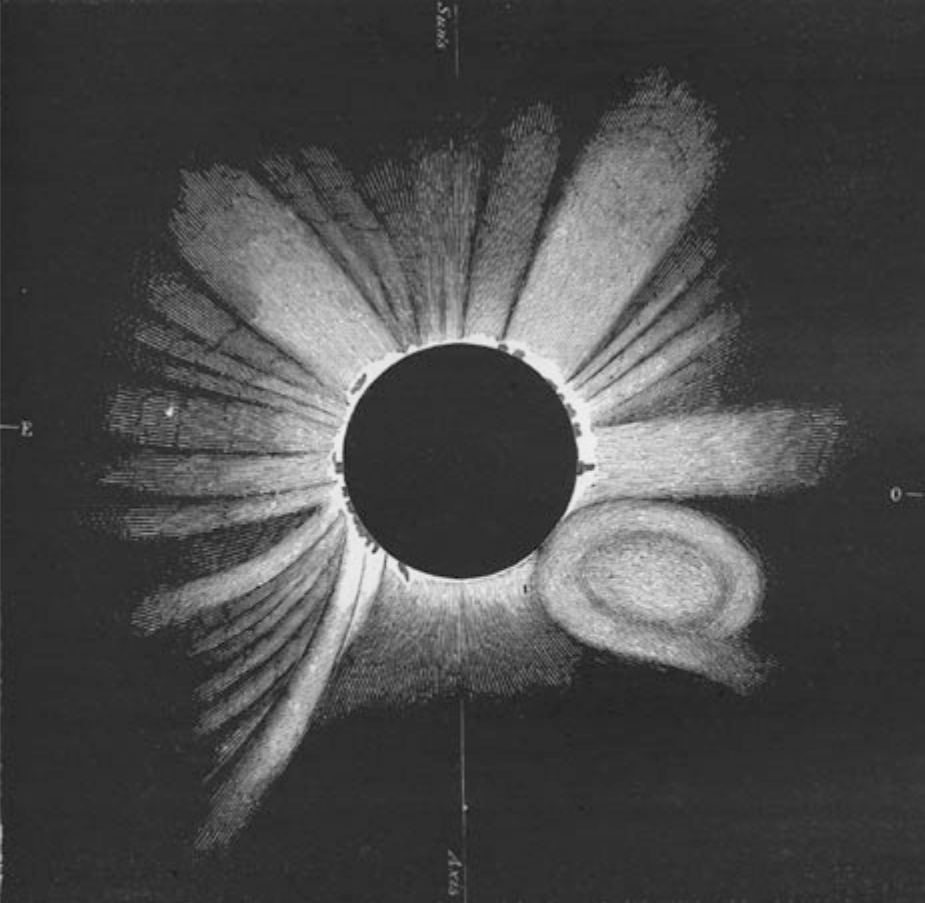
\includegraphics[width=0.7\linewidth]{imag/Primera_CME.png}
    \caption[Dibujo del eclipse de 1860 con la primera observación de una Eyección de Masa Coronal]{Dibujo del eclipse de 1860 registrado por Tempel, \cite{1879MmRAS..41..483.}. Se piensa que esta es la primera observación de una eyección de masa coronal.}
    \label{fig:PrimeraCME}
\end{figure}


\section{Ciclo Solar}
La actividad magnética solar, incluyendo las manchas solares y las CMEs, sigue un ciclo con un periodo de 11 años aproximadamente,\cite[e.g.,][]{hathaway-2015}. En cada ciclo, el campo magnético solar se invierte, pasando de un polo a otro.



\section{Viento solar}
Debido a la rotación del Sol, con un periodo aproximado de 27 días, el campo magnético interplanetario (IMF) llevado por el viento solar toma una forma de espiral doble de Arquímedes. Esto es porque el viento solar se libera radialmente de la superficie Solar, pero como el Sol está en rotación hace que las líneas de campo magnético se curven de tal forma que aparece una componente azimutal, perpendicular a la componente radial, por lo que esta curvatura se irá acumulando de tal forma que a medida que se aleje del Sol, la componente azimutal será más pronunciada que la componente radial. 
Se ha clasificado el viento solar en dos partes, el viento solar rápido ubicado en los polos del Sol, también asociado con los agujeros coronales y el lento ubicado sobre el ecuador del Sol. Sin embargo se ha encontrado un tercer tipo de viento solar, que es el viento solar límite que separa el rápido del lento. Se observó que el viento solar rápido tiene velocidades en el rango mayor a 675 kilómetros por segundo mientras que el viento solar lento está en el rango menor a los 500 kilómetros por segundo. El rango de velocidades entre el viento lento y el rápido corresponden al viento limítrofe o de frontera, es decir el rango entre 500 y 675 kilómetros por segundo., mostrado en \cite[e.g.,][]{stakhiv-2015}.
\begin{figure}
    \centering
    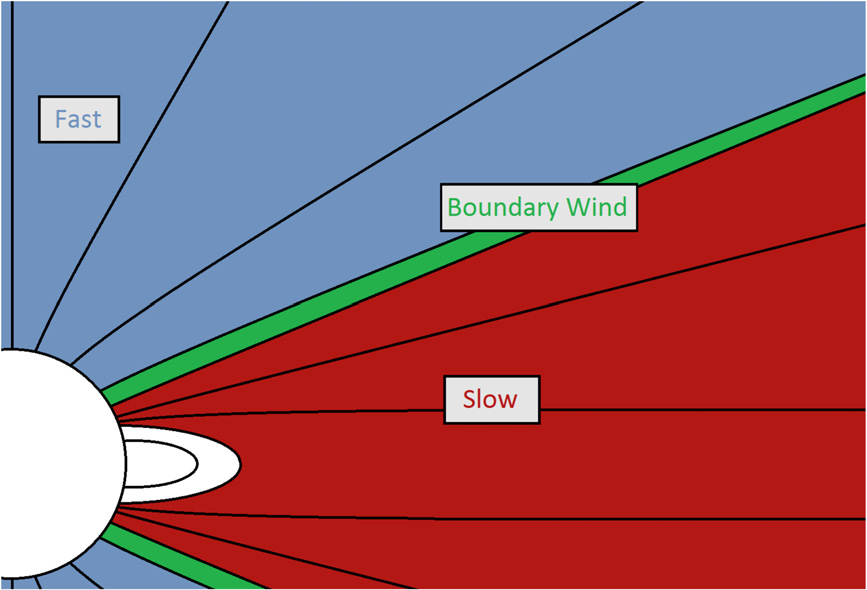
\includegraphics[width=0.7\linewidth]{Imagenes Mein/viento solar.png}
    \caption[Distribución del viento solar (lento, de interfaz, rápido) al rededor del Sol]{Diagrama del viento solar, en rojo el viento lento, en azul el viento rápido, en verde el viento de interfaz, extraído de \cite{stakhiv-2015}.}
    \label{fig:placeholder}
\end{figure}



\section{Magnetohidrodinámica}
La magnetohidrodinámica estudia el comportamiento de un fluido conductor inmerso en un espacio con campo magnético, dicho comportamiento se afectará así mismo, en \cite{cowling-1976} se muestra un texto en donde se condensa una introducción a la MHD, de ahí se tiene lo siguiente:

\subsection{Ecuaciones de la magnetohidrodinámica}

Se parte de las ecuaciones de Maxwell y de la hidrodinámica, llegando primero a la ecuación de continuidad hidrodinámica, que es de la forma:
\begin{equation}
\frac{\partial \rho}{\partial t}+\nabla(\rho v)=0
\end{equation}
Con $\rho$ la densidad y $v$ la velocidad del medio.
Las ecuaciones que constituyen la magnetohidrodinámica, además de la ya mencionada, son:
\begin{equation}
\nabla \times H=4\pi j,   ~~~~~~~\nabla \cdot j=0
\end{equation}


\begin{equation}
\nabla \times E=-\mu(\frac{\partial H}{\partial t}),~~~~~~\nabla \cdot H=0
\end{equation}

\begin{equation}
j=\sigma(E+\mu v\times H)
\end{equation}

\begin{equation}
\rho\frac{\partial v}{\partial t}+\rho v\cdot \nabla v=-\nabla p+\rho g+F+\mu j\times H
\end{equation}

Donde $j$ es la densidad de corriente, $H$ es el campo magnético, $E$ es el campo eléctrico, $g$ es la gravedad, $\sigma$ es la conductividad eléctrica, $v$ es la velocidad del medio, $p$ es la presión y $F$ es la fuerza de viscosidad que para un líquido viene dada por:
\begin{equation}
F=\rho \nu \nabla^{2}v
\end{equation}

Con $\nu$ la viscosidad cinemática.
Además, se debe considerar la energía interna por unidad de masa, dada por:
\begin{equation}
\rho\frac{dU}{dt}=\frac{p}{\rho}\frac{d\rho}{dt}+\lambda \nabla ^{2}T
\end{equation}

Donde $U$ es la energía interna por unidad de masa, $T$ es la temperatura y $\lambda$ es la conductividad térmica.

\subsection{Efectos electromagnéticos}

Con las ecuaciones anteriores es posible llegar a la ecuación:
\begin{equation}
\frac{\partial H}{\partial t}=\nabla \times(v\times H)+\frac{\nabla^{2}H}{4\pi \mu \sigma}
\end{equation}

Que es la variación del campo magnético en función de la velocidad del medio y del campo magnético mismo. Ya si consideramos el medio en reposo tenemos:
\begin{equation}
\frac{\partial H}{\partial t}=\frac{\nabla^{2}H}{4\pi \mu \sigma}
\end{equation}

Que es una ecuación de difusión, el coeficiente que acompaña al laplaciano del campo magnético se le conoce como la difusibilidad magnética: $\eta=\frac{1}{4\pi \mu \sigma}$
Las consecuencias de esta ecuación (para un medio estático) es que el campo magnético presenta un decrecimiento en un tiempo de decrecimiento que depende de la longitud por la que circula la corriente; para los conductores presentes en el cosmos, de gran tamaño, el tiempo de decrecimiento es, por ejemplo, de 15000 años para el campo magnético terrestre. 
El autor llega a encontrar que el tiempo de decrecimiento del campo magnético de una mancha solar es de 300 años, mientras que para el campo magnético del Sol es de $10^{10}$ años, todo esto en reposo.

La ecuación para un medio con velocidad pero con una conductividad muy grande ( o una resistencia despreciable) de tal forma que la difusibilidad magnética sea casi nula, es:
\begin{equation}
\frac{\partial H}{\partial t}=\nabla \times(v\times H)
\end{equation}

Esta ecuación es similar que la ecuación del torbellino, pero para el campo magnético. En el contexto del torbellino, la ecuación implica el arrastre de líneas de torbellino por el líquido. Según Alfvén, cuando la conductividad domina se pueden despreciar los términos de fuerzas inducidas, si la materia se mueve paralelo a las líneas de campo magnético, el material no modificará el campo en el cual se está moviendo, lo que implica que las líneas de campo están "congeladas"; si la materia se mueve en dirección perpendicular a las líneas de campo se encuentra que la materia en movimiento modifica el campo al arrastrar sus líneas de campo.

Ahora, se define el número de Reynolds magnético como:
\begin{equation}
R_{mag}=\frac{LV}{\eta}
\end{equation}

Donde $L$ es una longitud comparable con las dimensiones del campo y $V$ es una velocidad comparable con las velocidades reales. Este número nos indica que domina en el campo, si el arrastre de las líneas de campo o el decrecimiento del campo magnético. Por lo general, a nivel cósmico, lo que predomina es el arrastre de las líneas de campo magnético pero de forma lenta lo que lleva a algo como líneas de campo "congeladas", mientras que en un laboratorio en la Tierra predomina es el decrecimiento del campo magnético.

\subsection{Campos congelados}
La ecuación para campos congelados viene de las ecuaciones anteriores y tiene la forma:
\begin{equation}
\frac{\partial\left( \frac{H}{\rho} \right)}{\partial t}+v\cdot \nabla \left( \frac{H}{\rho} \right)=\left( \frac{H}{\rho}\cdot \nabla \right)v
\end{equation}

Ahora, si se presenta una perturbación en un tubo de lineas de fuerza, debido al arrastre de las líneas de campo, la magnitud del campo magnético y de la densidad presentarán una variación, pasando de ser $H$ y $\rho$ a ser $H'$ y $\rho'$, este cambio se puede ver en la ecuación:
\begin{equation}
\frac{H'}{\rho'}=\left( \frac{H}{\rho} \cdot \nabla\right)r'
\end{equation}
Siendo la forma integral de la ecuación anterior.

\subsection{Energía magnética}
Conociendo la densidad volumétrica de energía magnética: $\frac{\mu H^{2}}{8\pi}$ podemos encontrar la energía total del campo al integral en todo el volumen ocupado por el mismo:
\begin{equation}
W_{H}=\frac{1}{8\pi}\int_{V} \mu H^{2}dV
\end{equation}

Podemos determinar la variación de esta energía magnética de a través de:
\begin{equation}
\frac{d W_{H}}{dt}=\frac{1}{4\pi }\int \mu\{H\cdot \nabla(v\times H)+\eta H\cdot \nabla ^{2}H\}d \tau
\end{equation}

El segundo término de la parte derecha de la ecuación se puede reescribir como:
\begin{equation}
\frac{1}{4\pi}\int \mu \eta H\cdot \nabla ^{2}Hd\tau=-\int \frac{j^{2}}{\sigma}d\tau
\end{equation}

Por lo que este término representa la transformación de energía magnética a calor por efecto Joule a una razón de $\frac{j^{2}}{\sigma}$ por unidad de volumen. Ahora, el primer término de la parte derecha de la ecuación de la variación de la energía en el tiempo nos indica el trabajo realizado por la materia en el movimiento contra la fuerza magnética $j\times \mu H$. Esta fuerza magnética se puede escribir de la forma:
\begin{equation}
j\times \mu H=-\nabla\left( \frac{\mu H^{2}}{8\pi} \right)+\nabla \cdot\left( \mu  \frac{HH}{4\pi} \right)
\end{equation}

Esta ecuación nos dice que la fuerza magnética equivale a una \textbf{presión hidrostática} transversal (debida al primer término de la parte derecha, $\frac{\mu H^{2}}{8\pi}$) y a una \textbf{tensión magnética} a lo largo de las líneas de campo (debida al término de $\frac{\mu H^{2}}{4\pi}$), en otras palabras son las tensiones de Maxwell.
Cabe señalar que todo alargamiento de las líneas de fuerza lleva a un aumento de la energía magnética. Por otro lado, si las líneas de fuerza se separan, que es lo mismo a decir que la intensidad del campo magnético disminuye, la energía magnética disminuye.